\documentclass[10pt,a4paper]{report}
\usepackage[latin1]{inputenc}
\usepackage{amsmath}
\usepackage{amsfonts}
\usepackage{color}
\usepackage{amssymb}
\usepackage{graphicx}
\usepackage{fancyhdr}
\lhead{Introduction to \\ Computer Graphics}
\chead{Exercise 4}
\rhead{Kevin Serrano, 204141 \\ Gianni Scarnera, 195899}
\pagestyle{fancy}
\author{Kevin Serrano, Gianni Scarnera}
\title{Exercise 4}
\begin{document}
\maketitle

\section*{4.2   Scale and Translations}
Very simply, we scale the sun with its Scale factor (m\_sunScale) using scaleWorld. We then do the same for the earth and the moon using their scale factors and additionnally we translate them their correct position using their corresponding translation factors and translateWorld.
\begin{figure}[h!]
\caption{Scale and translations}
  \centering
    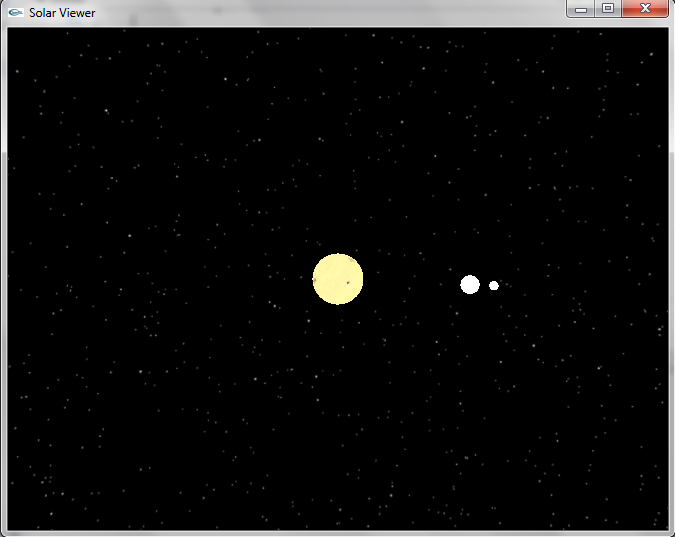
\includegraphics[width=0.7\textwidth]{im_4_2.png}
\end{figure}

\section*{4.3   Rotations}
First of all, we have to calculate the angle of rotation of each planet in one day. In the case of the Earth, the angle of rotation around its axis is given in degree by $\frac{360}{1} = 360$ degree per day. In radian it is $2 \pi$, and the angle of rotation around the sun in one day is given by $\frac{2 \pi}{365} $rad. We did same calculations for others planets. After that we have to multiply this angle per day with the days elapsed in our program to get the angle per loop.

After that we have to rotate the planet around the sun and themselves with the matrix of rotation around an axis in World coordinates, because we know that the sun is in the center of the universe in our model. So the sun rotates around itself, the Earth rotates around itself and around the sun, and the moon rotates around the sun and the Earth. The axis of rotation is $$axis = (0,1,0)$$ so now it is easy to calculate the rotations of each planet with the matrix $$rotateAroundAxisWorld(point,axis,angle)$$

\newpage 
\section*{4.4   Lighting and Textures}
First, we center the light using the origin of the sun and translateWorld on m\_light.

To compute the position of the light in camera coordinates we get the inverse of the camera transformation and we apply it to our light source position. Now, to calculate the indirect light intensity for the moon and earth we use this formula : $$((\mathbf{vectorToSun} \cdot \mathbf{vectorToOtherPLanet} + 1)/4) \cdot intesityOfSun$$
We also compute the camera coordinates for both the earth and the moon.

Then, in diffuse.vs, we compute the directions of the light and indirectlight like so :
$$lightDir = normalize(vertex - lightposition)$$
$$indirectLightDir = normalize(vertex - indirectlightposition)$$

In the fragment shader, we set a basecolor using the diffuseColor and the texture depending if useTexture is on or not. We then compute the intensities using this formula : $$I = I_p \cdot k_d \cdot (\mathbf{N} \cdot \mathbf{L})$$
for both color and indcolor. They are then put back together in finalcolor.

\begin{figure}[h!]
\caption{Screen shot of rotation. Diffuse model with direct and indirect light}
  \centering
    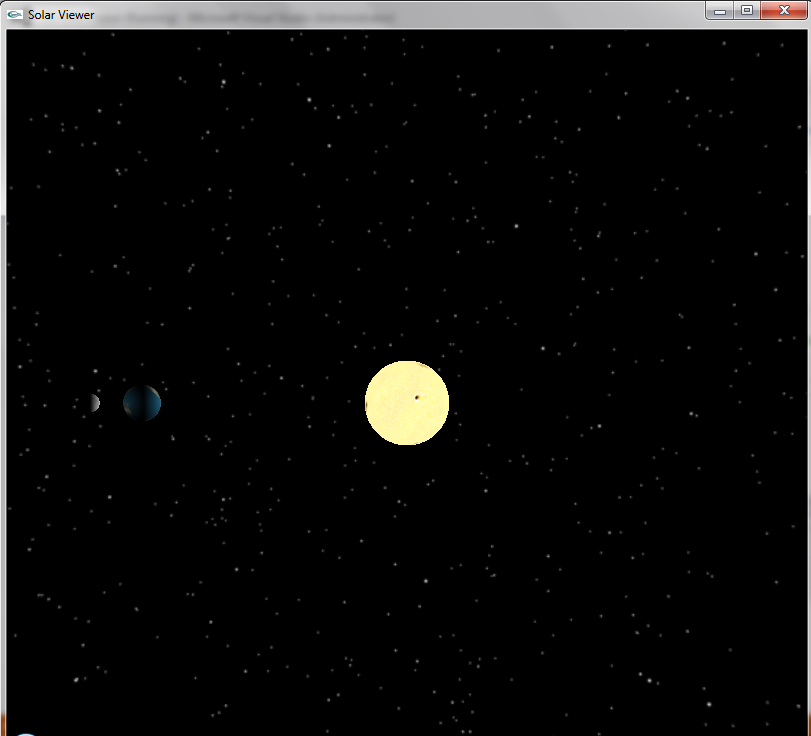
\includegraphics[width=0.9\textwidth]{im_4_3_4_4.png}
\end{figure}

\newpage

\section*{4.5   Geocentric Model}

First of all, if the geometric is available, we have to translate the camera from the sun to the Earth. It is easy if we use the vector sunToEarthVector and the translation matrix. Then We have to rotate the camera around the Earth with the same angle that the Earth around itself to get the impression that the Earth didn't move and all around moved (even the stars). Then we rendered all the scene and at the end we have to replace the camara to it's original position. So to do that we just did the inverse transformation, i.e first the rotation of the camera around the Earth with the negative angle and then the translation of the negative sunToEarthVector. This will simulate the fact that the Earth doesn't move and it is the center of the universe, but everything else will move. It moves very fast so we have to press the key down to slow down the animation.
\begin{figure}[h!]
\caption{Screen shot of geocentric model}
  \centering
    \includegraphics[width=0.9\textwidth]{im_4_5.png}
\end{figure}
\end{document}